% If you are using Word/Google Docs to write the report, you can ignore this file entirely!
% For LaTeX nerds, you can copy pasted this code to Overleaf to keep the template, and adjust it to your own work. 
\documentclass[12pt]{article}
	
\usepackage[margin=1in]{geometry}		% For setting margins
\usepackage{amsmath}				% For Math
\usepackage{amssymb} % For \mathbb
\usepackage{fancyhdr}				% For fancy header/footer
\usepackage{graphicx}	% For including figure/image
\renewcommand{\contentsname}{Table of Contents}
\usepackage{enumitem}
\usepackage{cancel}					% To use the slash to cancel out stuff in work
\usepackage[margin=0.25in]{geometry}
\usepackage{hyperref}
\usepackage{float}
\usepackage{multirow}
\usepackage{indentfirst}
\usepackage[american, siunitx]{circuitikz}
\usepackage{circuitikz}
\usepackage{lipsum}
\usepackage{setspace}
\usepackage{tikz, tcolorbox} 
\usepackage[dvipsnames]{xcolor}
\usepackage{listings}
\usepackage{xcolor}
\usepackage{fontspec}
\setmainfont{Times New Roman} % Use XeLaTex compiler to use this font. 



\pagestyle{fancy}
\fancyhead[LO,L]{Mark Le} % replace with your name!
\fancyhead[CO,C]{}
\fancyhead[RO,R]{\textbf{ELECENG 2EI4 Project 5 - Digital-to-Analog Converter}} 
\fancyfoot[LO,L]{}
\fancyfoot[CO,C]{\textbf{\thepage}}
\fancyfoot[RO,R]{}


%%%%%%%%%%%%%%%%%%%%%%

\spacing{1.25}
\begin{document}
    
    \begin{titlepage}
    \begin{center}
    \vspace*{\fill}

    {\LARGE \textbf{ELECENG 2EI4 - Electronic Devices \& Circuits I}\par}
    \vspace{2.5cm}

    {\LARGE\bfseries Project 5 - Digital-to-Analog Converter\par}
    \vspace{2.5cm}
    
    {\Large \textbf{Mark Le - 4005*****}\par} % replace with your name and student number
    \vspace{2.5cm}
    
    {\large \textbf{Instructor:} Dr. Yaser M. Haddara\par}
    \vspace{0.5cm}
    {\large \textbf{Term:} Winter 2026 \par} % winter 2027/28/29?
    \vspace{0.5cm}
    
    {\large \textbf{Submission Deadline:} Sunday, April 12, 2026\par}
    \end{center}

    \vspace*{\fill}

    \textbf{Statement of Originality:} As a future member of the engineering profession, the student is responsible for performing the required work in an honest manner, without plagiarism and cheating. Submitting this work with my name and student number is a statement and understanding that this work is my own and adheres to the Academic Integrity Policy of McMaster University and the Code of Conduct of the Professional Engineers of Ontario. Submitted by \textbf{Mark Le, lek37, 4005*****} % use your name, MacID, and student number. 

\end{titlepage}

    \newpage
    \tableofcontents

    \listoffigures

    \listoftables

    \newpage

	% from here, delete everything until before \end{document} and replace it with your own work
    \section{Summary}

    For this project, the implementation of a 3-bit digital-to-analog converter will be carried out with a full scale analog output voltage of 5V. The design utilized the functionality of an \textbf{inverting operational amplifier} (op-amp), and using binary-weighted input resistors to convert a 3-bit digital input as voltage into a corresponding analog output voltage. The whole project consists of three main parts: theoretical explanation of how the process of digital-to-analog conversion operates, the experimental result along with quantitative analysis of error that arises. Finally, a short discussion on how the error arises and an alternative design will also be carried out as well. 

    
    \section{Design}
    \subsection{Circuit Diagram}

    This is the overall block diagram of the DAC process used in this project: 
	\begin{figure}[H]
        \centering
        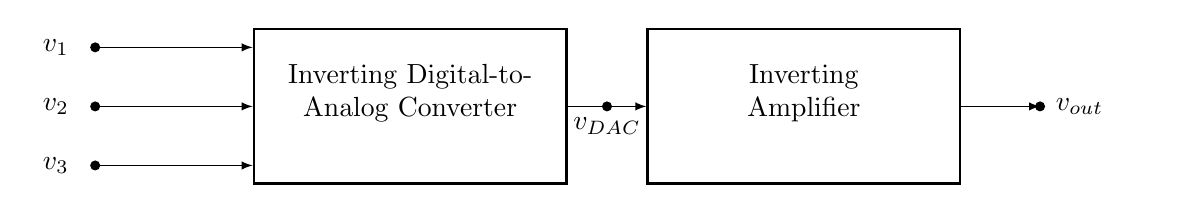
\begin{tikzpicture}[transform shape]
        	% Paths, nodes and wires:
        	\node[shape=rectangle, draw, line width=1pt, minimum width=3.965cm, minimum height=1.965cm] at (-10, 16.25){};
        	\node[shape=rectangle, minimum width=4.465cm, minimum height=1.34cm] at (-10, 16.313){} node[anchor=north, align=center, text width=4.077cm, inner sep=6pt] at (-10, 17){Inverting Digital-to-Analog Converter};
        	\draw[-latex] (-14, 17) -- (-12, 17);
        	\draw[-latex] (-14, 16.25) -- (-12, 16.25);
        	\draw[-latex] (-14, 15.5) -- (-12, 15.5);
        	\draw[-latex] (-8, 16.25) -- (-7, 16.25);
        	\node[shape=rectangle, draw, line width=1pt, minimum width=3.965cm, minimum height=1.965cm] at (-5, 16.25){};
        	\node[shape=rectangle, minimum width=2.465cm, minimum height=0.965cm] at (-5, 16.5){} node[anchor=north, align=center, text width=2.077cm, inner sep=6pt] at (-5, 17){Inverting Amplifier};
        	\draw[-latex] (-3, 16.25) -- (-2, 16.25);
        	\node[shape=rectangle, minimum width=0.715cm, minimum height=0.465cm](N1) at (-14.5, 17){} node[anchor=center] at (N1.text){$v_1$};
        	\node[shape=rectangle, minimum width=0.715cm, minimum height=0.465cm](N2) at (-14.5, 16.25){} node[anchor=center] at (N2.text){$v_2$};
        	\node[shape=rectangle, minimum width=0.715cm, minimum height=0.465cm](N3) at (-14.5, 15.5){} node[anchor=center] at (N3.text){$v_3$};
        	\node[circ] at (-14, 17){};
        	\node[circ] at (-14, 16.25){};
        	\node[circ] at (-14, 15.5){};
        	\node[circ] at (-2, 16.25){};
        	\node[circ] at (-7.5, 16.25){};
        	\node[shape=rectangle, minimum width=2.215cm, minimum height=0.715cm](N4) at (-7.5, 16){} node[anchor=center] at (N4.text){$v_{DAC}$};
        	\node[shape=rectangle, minimum width=2.215cm, minimum height=0.715cm](N5) at (-1.5, 16.25){} node[anchor=center] at (N5.text){$v_{out}$};
        \end{tikzpicture}
        \caption{DAC process block diagram}
    \end{figure}

    Here is the circuit diagram that is used for this project: 
    
    \begin{figure}[H]
        \centering
        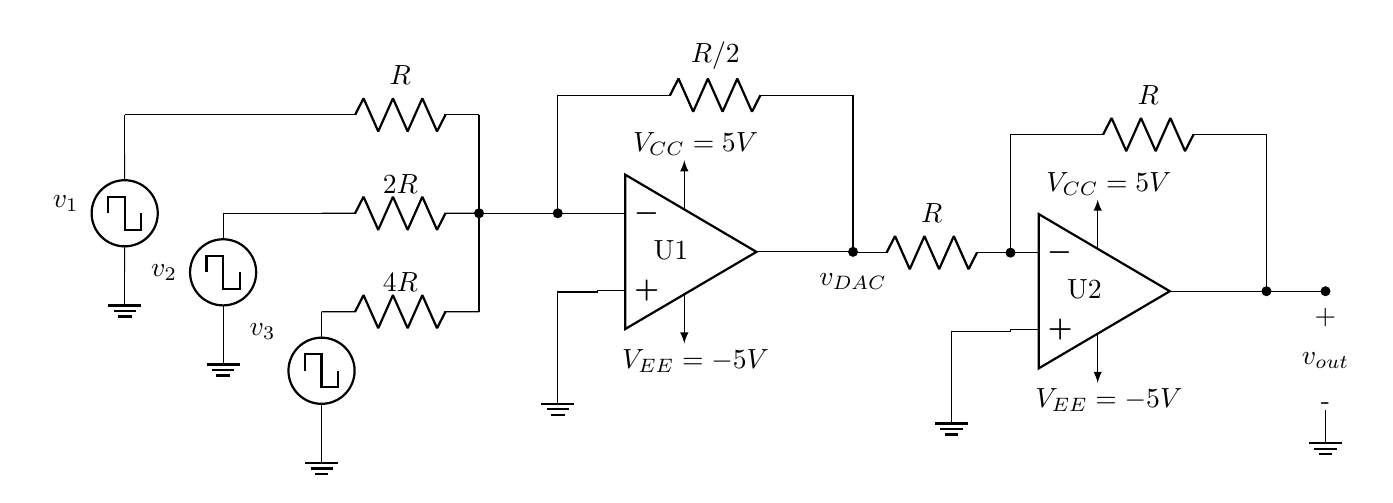
\begin{tikzpicture}[transform shape]
        	% Paths, nodes and wires:
        	\draw (-24.5, 27) to[square voltage source] (-24.5, 25.5);
        	\node[ground] at (-24.5, 25.5){};
        	\draw (-23.25, 26.25) to[square voltage source] (-23.25, 24.75);
        	\node[ground] at (-23.25, 24.75){};
        	\draw (-22, 25) to[square voltage source] (-22, 23.5);
        	\node[ground] at (-22, 23.5){};
        	\draw (-22, 27.5) to[american resistor] (-20, 27.5);
        	\draw (-22, 26.25) to[american resistor] (-20, 26.25);
        	\draw (-22, 25) to[american resistor] (-20, 25);
        	\draw (-24.5, 27.5) -- (-22, 27.5);
        	\draw (-23.25, 26.25) -- (-22, 26.25);
        	\draw (-22, 25.5) -| (-22, 25.5);
        	\node[op amp] at (-17.31, 25.76){};
        	\draw (-18.5, 26.25) -- (-20, 26.25);
        	\draw (-18.5, 25.27) |- (-19, 25.25) -| (-19, 24.25);
        	\node[ground] at (-19, 24.25){};
        	\draw (-18, 27.75) to[american resistor] (-16, 27.75);
        	\draw (-18, 27.75) -- (-19, 27.75) -| (-19, 26.25);
        	\draw (-16, 27.75) -- (-15.25, 27.75) -| (-15.25, 25.75) |- (-16.12, 25.76);
        	\node[circ] at (-19, 26.25){};
        	\node[circ] at (-20, 26.25){};
        	\node[circ] at (-15.25, 25.76){};
        	\node[shape=rectangle, minimum width=0.965cm, minimum height=0.715cm] at (-17.5, 25.75){} node[anchor=north west, align=left, text width=0.577cm, inner sep=6pt] at (-18, 26.125){U1};
        	\draw[-latex] (-17.393, 26.299) -- (-17.393, 26.924);
        	\draw[-latex] (-17.393, 25.221) -- (-17.393, 24.596);
        	\draw (-15.25, 25.75) to[american resistor] (-13.25, 25.75);
        	\node[op amp] at (-12.06, 25.26){};
        	\draw (-12.5, 27.25) to[american resistor] (-10.5, 27.25);
        	\draw (-13.25, 25.75) -| (-13.25, 27.25) -- (-12.5, 27.25);
        	\draw (-10.5, 27.25) -- (-10, 27.25) -| (-10, 25.25) |- (-10.87, 25.26);
        	\draw (-13.25, 24.77) |- (-14, 24.75) -| (-14, 24);
        	\node[ground] at (-14, 24){};
        	\draw[-latex] (-12.143, 25.799) -- (-12.143, 26.424);
        	\draw[-latex] (-12.143, 24.721) -- (-12.143, 24.096);
        	\node[shape=rectangle, minimum width=0.965cm, minimum height=0.715cm] at (-12.25, 25.25){} node[anchor=north west, align=left, text width=0.577cm, inner sep=6pt] at (-12.75, 25.625){U2};
        	\draw (-10, 25.26) -| (-9.25, 25.25);
        	\node[circ] at (-9.25, 25.26){};
        	\node[circ] at (-10, 25.26){};
        	\node[circ] at (-13.25, 25.75){};
        	\node[shape=rectangle, minimum width=0.965cm, minimum height=0.715cm](N1) at (-25.25, 26.375){} node[anchor=center] at (N1.text){$v_1$};
        	\node[shape=rectangle, minimum width=0.965cm, minimum height=0.715cm](N2) at (-24, 25.5){} node[anchor=center] at (N2.text){$v_2$};
        	\node[shape=rectangle, minimum width=0.965cm, minimum height=0.715cm](N3) at (-22.75, 24.75){} node[anchor=center] at (N3.text){$v_3$};
        	\node[shape=rectangle, minimum width=0.965cm, minimum height=0.715cm](N4) at (-21, 28){} node[anchor=center] at (N4.text){$R$};
        	\node[shape=rectangle, minimum width=0.965cm, minimum height=0.715cm](N5) at (-21, 26.625){} node[anchor=center] at (N5.text){$2R$};
        	\node[shape=rectangle, minimum width=0.965cm, minimum height=0.715cm](N6) at (-21, 25.375){} node[anchor=center] at (N6.text){$4R$};
        	\node[shape=rectangle, minimum width=0.965cm, minimum height=0.715cm](N7) at (-17, 28.25){} node[anchor=center] at (N7.text){$R/2$};
        	\node[shape=rectangle, minimum width=0.965cm, minimum height=0.715cm](N8) at (-14.25, 26.25){} node[anchor=center] at (N8.text){$R$};
        	\node[shape=rectangle, minimum width=0.965cm, minimum height=0.715cm](N9) at (-11.5, 27.75){} node[anchor=center] at (N9.text){$R$};
        	\node[ground] at (-9.25, 23.75){};
        	\node[shape=rectangle, minimum width=0.965cm, minimum height=0.715cm](N10) at (-9.25, 24.375){} node[anchor=center] at (N10.text){$v_{out}$};
        	\node[shape=rectangle, minimum width=0.965cm, minimum height=0.715cm] at (-9.25, 24.885){} node[anchor=north, align=center, text width=0.577cm, inner sep=6pt] at (-9.25, 25.26){+};
        	\node[shape=rectangle, minimum width=0.965cm, minimum height=0.715cm] at (-9.25, 23.75){} node[anchor=north, align=center, text width=0.577cm, inner sep=6pt] at (-9.25, 24.125){-};
        	\node[shape=rectangle, minimum width=0.965cm, minimum height=0.715cm](N11) at (-17.25, 27.125){} node[anchor=center] at (N11.text){$V_{CC}=5V$};
        	\node[shape=rectangle, minimum width=0.965cm, minimum height=0.715cm](N12) at (-12, 26.625){} node[anchor=center] at (N12.text){$V_{CC}=5V$};
        	\node[shape=rectangle, minimum width=0.965cm, minimum height=0.715cm](N13) at (-17.25, 24.375){} node[anchor=center] at (N13.text){$V_{EE}=-5V$};
        	\node[shape=rectangle, minimum width=0.965cm, minimum height=0.715cm](N14) at (-12, 23.875){} node[anchor=center] at (N14.text){$V_{EE}=-5V$};
        	\draw (-24.5, 27) -| (-24.5, 27.5);
        	\draw (-20, 27.5) -| (-20, 26.25);
        	\draw (-20, 25) -| (-20, 26.25);
            \node[shape=rectangle, minimum width=0.965cm, minimum height=0.715cm](N15) at (-15.25, 25.385){} node[anchor=center] at (N15.text){$v_{DAC}$};
        \end{tikzpicture}
        \caption{DAC circuit schematics}
    \end{figure}

    \newpage
    \subsection{Circuit Operations}

    For this circuit, we will assume that the operational amplifier used (both U1 and U2) is ideal. The characteristics of ideal op-amp includes: 

    \begin{itemize}
        \item Very high intrinsic gain, \(A_0\), and it is assumed that \(A_0 \to \infty \). [1]
        \item Very high input resistance, \(R_i\), and very small output resistance \(R_o\). It is assumed that \(R_i \to \infty\) and \(R_o=0\) [1]
    \end{itemize}

    That leads to: 
    \begin{itemize}
        \item The input current to the two op-amp terminals. inverting (-) and non-inverting (+) are zero [1]
        \item The input voltages to the two op-amp terminals, inverting (-) and non-inverting (+) are equals to each other [1]
    \end{itemize}

    \begin{equation*}
        \begin{cases}
            V_-=V_+ \\ 
            I_-=I_+=0A
        \end{cases}
    \end{equation*}

    In the circuit on section 2.1, there are three voltage inputs: \(v_1,v_2,v_3\) represents the binary input, HIGH and LOW. For a LOW logic input (binary 0), the input is represented as 0V DC input. For a HIGH logic input (binary 1), the input is represented as 5V DC input. Each digital input is applied at three inputs \(v_1,v_2,v_3\) through a scaled resistor value of \(R,2R,4R\), respectively. Thus, each input resistor branch also produce a scaled current to the summing node (input node to the inverting op-amp input). The input \(v_1\) connected through resistor \(R\) drives the most amount of current to the summing node, since, so it acts like a most significant bit (LSB) in the binary input. Conversely, the input \(v_3\) through resistor of value \(4R\) drives the least amount of current, and thus acts like a least significant bit (LSB) in the binary input. [3]


    The op-amp U1 with the feedback resistor \(R/2\) keeps the inverting input (-) approximately 0V  through negative feedback. This resistor also control the internal gain of the first op-amp (will be proved quantitatively in the calculation). As discussed, idealized op-amp model does not draw any current into the inverting/non-inverting input, the current from the summing node flows through the feedback resistor, producing an converted analog voltage given the input voltage from \(v_1,v_2,v_3\). Since there are 8 input combinations from the three inputs, there will be 8 corresponding voltage level at the output. [1]


    Since the digital input combinations goes through the inverting input terminal (-), the output voltage will be inverted as well at analog-converted voltage \(v_{DAC}\). That mean the positive-valued input at \(v_1,v_2,v_3\) will produce a corresponding output at \(v_{DAC}\) with a negative sign. To invert the voltage, a op-amp U2 is used as a \textbf{inverting voltage amplifier} with negative gain to revert the sign of \(v_{DAC}\). 


    \subsection{Calculations}

     In overall, the circuit transform a digital input at \(v_1,v_2,v_3\) into corresponding analog voltage output at \(v_{out}\). For this project, we will be using a reference voltage, \(V_{ref}\) of 5 V. The resolution of the conversion is related to the number of bits. In this case, there are 3 bits, and the resolution can be computed by taking the reference voltage and divide by \(2^n\), where \(n\) is the number of bits. [3]
     \[\text{Resolution}=\frac{V_{ref}}{2^n}=\frac{5V}{2^3}=0.625V\]

     Next, the full-scale output voltage is calculated by setting all inputs to HIGH (1), defined by multiplying the resolution to the maximum binary input [3]
     \[V_{FS}=\text{Resolution} \times (2^n-1)=0.625(7)=4.375V\]

     Label the node on the circuit appropriately: 
    \begin{figure}[H]
        \centering
            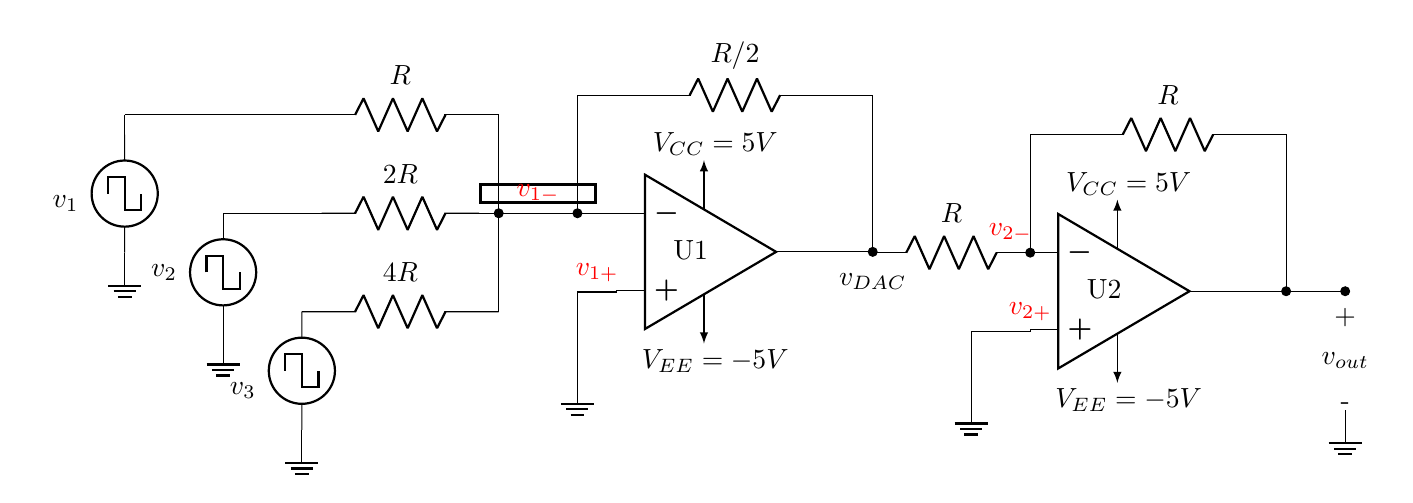
\begin{tikzpicture}[transform shape]
            	% Paths, nodes and wires:
            	\draw (-24.75, 27.25) to[square voltage source] (-24.75, 25.75);
            	\node[ground] at (-24.75, 25.75){};
            	\draw (-23.5, 26.25) to[square voltage source] (-23.5, 24.75);
            	\node[ground] at (-23.5, 24.75){};
            	\draw (-22.5, 25) to[square voltage source] (-22.5, 23.5);
            	\node[ground] at (-22.5, 23.5){};
            	\draw (-22.25, 27.5) to[american resistor] (-20.25, 27.5);
            	\draw (-22.25, 26.25) to[american resistor] (-20.25, 26.25);
            	\draw (-22.5, 25) to[american resistor] (-20, 25);
            	\draw (-24.75, 27.5) -- (-22, 27.5);
            	\draw (-23.5, 26.25) -- (-22, 26.25);
            	\draw (-22, 25.5) -| (-22, 25.5);
            	\node[op amp] at (-17.31, 25.76){};
            	\draw (-18.5, 26.25) -- (-20, 26.25);
            	\draw (-18.5, 25.27) |- (-19, 25.25) -| (-19, 24.25);
            	\node[ground] at (-19, 24.25){};
            	\draw (-18, 27.75) to[american resistor] (-16, 27.75);
            	\draw (-18, 27.75) -- (-19, 27.75) -| (-19, 26.25);
            	\draw (-16, 27.75) -- (-15.25, 27.75) -| (-15.25, 25.75) |- (-16.12, 25.76);
            	\node[circ] at (-19, 26.25){};
            	\node[circ] at (-20, 26.25){};
            	\node[circ] at (-15.25, 25.76){};
            	\node[shape=rectangle, minimum width=0.965cm, minimum height=0.715cm] at (-17.5, 25.75){} node[anchor=north west, align=left, text width=0.577cm, inner sep=6pt] at (-18, 26.125){U1};
            	\draw[-latex] (-17.393, 26.299) -- (-17.393, 26.924);
            	\draw[-latex] (-17.393, 25.221) -- (-17.393, 24.596);
            	\draw (-15.25, 25.75) to[american resistor] (-13.25, 25.75);
            	\node[op amp] at (-12.06, 25.26){};
            	\draw (-12.5, 27.25) to[american resistor] (-10.5, 27.25);
            	\draw (-13.25, 25.75) -| (-13.25, 27.25) -- (-12.5, 27.25);
            	\draw (-10.5, 27.25) -- (-10, 27.25) -| (-10, 25.25) |- (-10.87, 25.26);
            	\draw (-13.25, 24.77) |- (-14, 24.75) -| (-14, 24);
            	\node[ground] at (-14, 24){};
            	\draw[-latex] (-12.143, 25.799) -- (-12.143, 26.424);
            	\draw[-latex] (-12.143, 24.721) -- (-12.143, 24.096);
            	\node[shape=rectangle, minimum width=0.965cm, minimum height=0.715cm] at (-12.25, 25.25){} node[anchor=north west, align=left, text width=0.577cm, inner sep=6pt] at (-12.75, 25.625){U2};
            	\draw (-10, 25.26) -| (-9.25, 25.25);
            	\node[circ] at (-9.25, 25.26){};
            	\node[circ] at (-10, 25.26){};
            	\node[circ] at (-13.25, 25.75){};
            	\node[shape=rectangle, minimum width=0.965cm, minimum height=0.715cm](N1) at (-25.5, 26.375){} node[anchor=center] at (N1.text){$v_1$};
            	\node[shape=rectangle, minimum width=0.965cm, minimum height=0.715cm](N2) at (-24.25, 25.5){} node[anchor=center] at (N2.text){$v_2$};
            	\node[shape=rectangle, minimum width=0.965cm, minimum height=0.715cm](N3) at (-23.25, 24){} node[anchor=center] at (N3.text){$v_3$};
            	\node[shape=rectangle, minimum width=0.965cm, minimum height=0.715cm](N4) at (-21.25, 28){} node[anchor=center] at (N4.text){$R$};
            	\node[shape=rectangle, minimum width=0.965cm, minimum height=0.715cm](N5) at (-21.25, 26.75){} node[anchor=center] at (N5.text){$2R$};
            	\node[shape=rectangle, minimum width=0.965cm, minimum height=0.715cm](N6) at (-21.25, 25.5){} node[anchor=center] at (N6.text){$4R$};
            	\node[shape=rectangle, minimum width=0.965cm, minimum height=0.715cm](N7) at (-17, 28.25){} node[anchor=center] at (N7.text){$R/2$};
            	\node[shape=rectangle, minimum width=0.965cm, minimum height=0.715cm](N8) at (-14.25, 26.25){} node[anchor=center] at (N8.text){$R$};
            	\node[shape=rectangle, minimum width=0.965cm, minimum height=0.715cm](N9) at (-11.5, 27.75){} node[anchor=center] at (N9.text){$R$};
            	\node[ground] at (-9.25, 23.75){};
            	\node[shape=rectangle, minimum width=0.965cm, minimum height=0.715cm](N10) at (-9.25, 24.375){} node[anchor=center] at (N10.text){$v_{out}$};
            	\node[shape=rectangle, minimum width=0.965cm, minimum height=0.715cm] at (-9.25, 24.885){} node[anchor=north, align=center, text width=0.577cm, inner sep=6pt] at (-9.25, 25.26){+};
            	\node[shape=rectangle, minimum width=0.965cm, minimum height=0.715cm] at (-9.25, 23.75){} node[anchor=north, align=center, text width=0.577cm, inner sep=6pt] at (-9.25, 24.125){-};
            	\node[shape=rectangle, minimum width=0.965cm, minimum height=0.715cm](N11) at (-17.25, 27.125){} node[anchor=center] at (N11.text){$V_{CC}=5V$};
            	\node[shape=rectangle, minimum width=0.965cm, minimum height=0.715cm](N12) at (-12, 26.625){} node[anchor=center] at (N12.text){$V_{CC}=5V$};
            	\node[shape=rectangle, minimum width=0.965cm, minimum height=0.715cm](N13) at (-17.25, 24.375){} node[anchor=center] at (N13.text){$V_{EE}=-5V$};
            	\node[shape=rectangle, minimum width=0.965cm, minimum height=0.715cm](N14) at (-12, 23.875){} node[anchor=center] at (N14.text){$V_{EE}=-5V$};
            	\draw (-24.75, 27) -| (-24.75, 27.5);
            	\draw (-20, 27.5) -| (-20, 26.25);
            	\draw (-20, 25) -| (-20, 26.25);
            	\node[shape=rectangle, minimum width=0.965cm, minimum height=0.715cm](N15) at (-15.25, 25.385){} node[anchor=center] at (N15.text){$v_{DAC}$};
            	\node[shape=rectangle, draw, line width=1pt, minimum width=1.465cm, minimum height=-0.035cm] at (-19.5, 26.5){};
            	\node[shape=rectangle, draw, line width=1pt, minimum width=1.465cm, minimum height=-0.035cm] at (-19.5, 26.5){};
            	\draw (-20, 27.5) -- (-20.25, 27.5);
            	\draw (-20.25, 26.25) -- (-20, 26.25);
            	\node[shape=rectangle, minimum width=0.965cm, minimum height=0.715cm](N16) at (-19.5, 26.5){} node[anchor=center] at (N16.text){\textcolor{rgb,255:red,255;green,0;blue,0}{$v_{1-}$}};
            	\node[shape=rectangle, minimum width=0.965cm, minimum height=0.715cm](N17) at (-18.75, 25.5){} node[anchor=center] at (N17.text){\textcolor{rgb,255:red,255;green,0;blue,0}{$v_{1+}$}};
            	\node[shape=rectangle, minimum width=0.965cm, minimum height=0.715cm](N18) at (-13.25, 25){} node[anchor=center] at (N18.text){\textcolor{rgb,255:red,255;green,0;blue,0}{$v_{2+}$}};
            	\node[shape=rectangle, minimum width=0.965cm, minimum height=0.715cm](N19) at (-13.5, 26){} node[anchor=center] at (N19.text){\textcolor{rgb,255:red,255;green,0;blue,0}{$v_{2-}$}};
        \end{tikzpicture}
        \caption{Circuit Schematics with labeled nodes}
    \end{figure}

    Derivation of \(v_{DAC}\):


    KCL at node \(v_{1-}\): 

    \[\frac{v_{-1}-v_1}{R}+\frac{v_{-1}-v_2}{2R}+\frac{v_{-1}-v_3}{4R}+\frac{v_{-1}-v_{DAC}}{R/2}=0\]
    \[4(v_{-1}-v_1)+2(v_{-1}-v_2)+v_{-1}-v_3=-8(v_{-1}-v_{DAC})\]
    Since \(v_{-1}=v_{+1}=0V\), assuming ideal op-amp model:
    \[-4v_1-2v_2-v_3=8v_{DAC}\]
    \[v_{DAC}=-\frac{1}{2}v_1-\frac{1}{4}v_2-\frac{1}{8}v_3\]

    KCL at node \(v_{-2}\):
    \[\frac{v_{-2}-v_{DAC}}{R}+\frac{v_{-2}-v_{out}}{R}=0\]
    \[v_{-2}-v_{DAC}+v_{-2}-v_{out}=0\]

    Since \(v_{-2}=v_{+2}=0V\):
    \[-v_{DAC}=v_{out}\]
    \[\therefore v_{out}=\frac{1}{2}v_1+\frac{1}{4}v_2+\frac{1}{8}v_3\]

    If we treat \(v_1,v_2,v_3\) as binary number input (0 and 1), then the correct formula would be: 
    \[v_{out}=V_{ref}\Big( \frac{1}{2} v_1 + \frac{1}{4}v_2+\frac{1}{8}v_3\Big)\]

    This following tables list all the analog output voltage (expected) based on the digital input: 
    \begin{table}[H]
        \centering
        \begin{tabular}{|c|c|c|c|c|}
            \hline
            \multicolumn{3}{|c|}{\textbf{Inputs}} & \textbf{Decimals Value} & \(v_{out}\) (V) \\ \hline
            \(v_1\) & \(v_2\) & \(v_3\) &  & \\ \hline
            0 & 0 & 0 & 0 & 0 \\ \hline
            0 & 0 & 1 & 1 & 0.625 \\ \hline
            0 & 1 & 0 & 2 & 1.25 \\ \hline
            0 & 1 & 1 & 3 & 1.875 \\ \hline
            1 & 0 & 0 & 4 & 2.5 \\ \hline
            1 & 0 & 1 & 5 & 3.125 \\ \hline
            1 & 1 & 0 & 6 & 3.75 \\ \hline
            1 & 1 & 1 & 7 & 4.375 \\ \hline
        \end{tabular}
        \caption{3-bit Digital-to-Analog voltage conversion}
    \end{table}
     

     
    \subsection{Reference}

    The circuit schematic is the result of two schematics combinations. The digital-to-analog converter circuit was consulted through \textbf{COMPENG 2CF3 - Circuit \& Waves} course, at \textbf{Lecture 1 \& 2 - Operational Amplifiers}, taught by Dr. Natalia Nikolova. The resistor values are consulted through \textit{Electronics Tutorials: Digital to Analogue Converter} [2]. The inverting voltage amplifier was also consulted on the course \textbf{COMPENG 2CF3} as well. 


    \section{Measurement \& Analysis}
    \subsection{Breadboard Circuit}

    After careful consideration on limitation of the 2CI4 and 2EI4 component kits, I decide to use \(R=2.5k\Omega\). Note that the resistor between the node \(v_{DAC}\) and \(v_{-2}\) on my breadboard have \(2.495k\Omega\) instead of \(2.5k\Omega\) resistance due to lack of resistors, by connecting two \(4.99k\Omega\) resistors in parallel.  

    \begin{figure}[H]
        \centering
        \includegraphics[width=0.8\linewidth]{Image (5).jpg}
        \caption{Breadboard circuit schematics}
    \end{figure}

    \subsection{Digital Input Generations}

    To generate the input for the circuit, I configured the \texttt{Supplies} channel in the Waveform software as following:
    \begin{itemize}
        \item Positive Supply (V+): 5V. This is connected from the V+ probe of the AD3 to the common positive rail of the breadboard, to the \(V_{+}\) pin of the LM662CN op-amps, 
        \item Negative Supply (V-): -5V. This is connected straight from the V- probe of the AD3 to the \(V_{-}\) pin of the LM662CN op-amps. 
    \end{itemize}

    \begin{figure}[H]
        \centering
        \includegraphics[width=1\linewidth]{Screenshot 2026-04-12 162640.png}
        \caption{DC power supplies configurations}
    \end{figure}

    Additionally, the GND probe from the AD3 is connected to the negative rail of the breadboard. The digital input \(v_1,v_2,v_3\) are placed at the positive rail (5V) or the negative rail (0V) correspond to logic HIGH (1) or logic LOW (0), respectively, to generate a 3-bit binary input combination. 

    
    \subsection{Transfer Characteristics}

    The table below shows the output read from the AD3. Digital input of 1 is 5V, 0 is GND 

    \begin{table}[H]
        \centering
        \begin{tabular}{|c|c|c|c|c|c|}
            \hline
            \multicolumn{3}{|c|}{\textbf{Inputs}} & \textbf{Decimals Value} & \(v_{theoretical}\) (V) & \(v_{actual}\) (V) \\ \hline
            \(v_1\) & \(v_2\) & \(v_3\) &  & & \\ \hline
            0 & 0 & 0 & 0 & 0 & 0.036 \\ \hline
            0 & 0 & 1 & 1 & 0.625 & 0.653 \\ \hline
            0 & 1 & 0 & 2 & 1.25 & 1.236 \\ \hline
            0 & 1 & 1 & 3 & 1.875 & 1.873 \\ \hline
            1 & 0 & 0 & 4 & 2.5 & 2.484 \\ \hline
            1 & 0 & 1 & 5 & 3.125 & 3.121 \\ \hline
            1 & 1 & 0 & 6 & 3.75 & 3.733 \\ \hline
            1 & 1 & 1 & 7 & 4.375 & 4.345 \\ \hline
        \end{tabular}
        \caption{Theoretical versus experimental results}
    \end{table}

    \newpage
    The figure below demonstrates the transfer characteristics:

    \begin{figure}[H]
        \centering
        \includegraphics[width=0.9\linewidth]{Screenshot 2026-04-12 165059.png}
        \caption{Transfer Characteristics}
        \label{fig:placeholder}
    \end{figure}

    The transfer characteristics shown in Figure 6 is shown as a staircase shaped since the digital input is taken instead of analog input, with the decimal value equivalent of the 3-bit input code. The blue plot represent the theoretical transfer characteristics of the circuit, and the red plot represents a actual transfer characteristics by plotting the output analog voltage versus digital input, and those two plots are close to each other, which is expected for a digital-to-analog converter circuit, thus confirming proper DAC operation. 
    
    

    \subsection{Error Measurement}

    \textbf{Gain error}: this quantity represents the percentage error of the actual full-scaled voltage versus the expected full-scaled voltage. For this project, \[V_{FS, theoretical}=4.375V\], and \[V_{FS, actual}=V_{out,111}-V_{out,000}=4.345-0.036=4.309V\]. The gain error (\(GE\)) equation is: 

    \[GE=\Big|\frac{v_{FS,actual}-v_{FS,theoretical}}{v_{FS,theoretical}}\Big| \times 100\%\]
    \[GE=\Big|\frac{4.309V-4.375V}{4.375V}\Big| \times 100\%=1.508\%\]


    \textbf{Maximum differential non-linearity}: this quantity represents the maximum percentage error of the actual step size when the binary input is increment by 1, compared to the expected resolution of 0.625 V. The table below shows the step size of each output voltage as the digital input increments. 

    \begin{table}[H]
        \centering
        \begin{tabular}{|c|c|c|c|c|c|c|}
            \hline
            \multicolumn{3}{|c|}{\textbf{Inputs}} & \textbf{Decimals Value} & \(v_{theoretical}\) (V) & \(v_{actual}\) (V) & \(\Delta V_{actual}\) (V) \\ \hline
            \(v_1\) & \(v_2\) & \(v_3\) &  & & &  \\ \hline
            0 & 0 & 0 & 0 & 0 & 0.036 & N/A \\ \hline
            0 & 0 & 1 & 1 & 0.625 & 0.653 & 0.617 \\ \hline
            0 & 1 & 0 & 2 & 1.25 & 1.236 & \textcolor{red}{0.583}\\ \hline
            0 & 1 & 1 & 3 & 1.875 & 1.873 & 0.637 \\ \hline
            1 & 0 & 0 & 4 & 2.5 & 2.484 & 0.611 \\ \hline
            1 & 0 & 1 & 5 & 3.125 & 3.121 & 0.637 \\ \hline
            1 & 1 & 0 & 6 & 3.75 & 3.733 & 0.612\\ \hline
            1 & 1 & 1 & 7 & 4.375 & 4.345 & 0.612 \\ \hline
        \end{tabular}
        \caption{Differential non-linearity as digital input increments}
    \end{table}

    As shown in the table, the change from input 001 (decimal 1) to 010 (decimal 2) deviates the most from the expected resolution of 0.625 V. Therefore, the maximum differential non-linearity error is: 

    \[DNL_{max}=\Bigg|\frac{0.583V-0.625V}{0.625V}\Bigg| \times 100\%=\boxed{6.72\%}\]

    \textbf{Offset error:} is the output error when the input code is 000. The offset error is measured by taking the measured output voltage when the input is 000 (decimal 0). Table 3 shows that the result came out to be 0.036 V. Therefore, the offset error is 0.036 V. 
    \newpage
    \section{Discussion}
    

    \subsection{Error Analysis}

    There are various sources that leads to the discrepancies that leads to gain error, differential non-linearity error and offset error. Some noticeable errors includes:

    \begin{itemize}
        \item \textbf{Ideal op-amps conditions:} the assumption on section 2.1 tells that the intrinsic gain \(A_0\) and input resistance are close to \(\infty\), and output resistance is close to 0. However, this is not true for the physical op-amp used for this project. The datasheet tells that the intrinsic gain is \(A_0=2 \times 10^6\), input resistance of \(R_i>1T\Omega\), and output resistance is non-zero [2] This leads to the assumption on section 2.1 becomes untrue, which leads to the discrepancies for the output measurement. 

        \item \textbf{Component tolerance}: each resistors in the 2CI4/2EI4 kits has a tolerance rate of \(\pm 5\%\). This means the actual resistor values is \(\pm 5\%\) difference from the expected values. Since the output voltage depends heavily on the resistor values, the measurement came out to be slightly deviated from the expected values. 
    \end{itemize}

    \subsection{Design Justifications}

    For this project, the binary-weighted resistor digital-to-analog converter (DAC) is used to implement the circuit due to its simple configuration and easy to debug. Additionally, this topology offers a easy understanding of the contribution of each input bit easy, since each resistor directly represents its binary significance. While the R-2R ladder topology is known as a better configuration due to its scalability (only use 2 resistor values), this configuration would not be feasible because it requires more resistors to implement, since each inputs requires 2 resistors instead of 1, and each resistor requires complex series or parallel combination, which makes it very hard to track the nodes and debug. 

    \newpage
    \begin{thebibliography}{9}

    \bibitem{N. Nikolova}
        N. Nikolova, ``COMPENG 2CF3: Lecture 1 \& 2 - Operational Amplifiers'' 
        . Available: https://avenue.cllmcmaster.ca/d2l/le/lessons/758461/topics/5494405. Accessed Apr, 12. 2026.

    \bibitem{Texas Instruments}
        Texas Instruments, ``LMC66x CMOS Dual Operational Amplifiers'' 
        [Online]. Available: https://www.digikey.ca/en/products/detail/texas-instruments/LMC662CN-NOPB/148218?gclsrc=aw.ds\&gad\_source=1\&gad\_campaignid=23536462204\&gbraid=0AAAAADrbLlgXH \\ wmg0AvNOoXGC9cO93fE6\&gclid=CjwKCAjwhe3OBhABEiwA6392zAXr0hcvvno78B4Rj-MABi35RwadVayYvlex5LD3hdQVZzyV\_HC5cxoCth4QAvD\_BwE. Accessed Apr, 12. 2026

    \bibitem{Electronics Tutorials}
    Electronics Tutorials, ``Binary Weighted Digital to Analogue Converter'' 
    [Online]. Available: https://www.electronics-tutorials.ws/combination/digital-to-analogue-converter.html. Accessed Apr, 12. 2026

    \end{thebibliography} 

\end{document}
